

\subsection{SPC evaluation}
\label{sec:eval_spc}

\subsubsection{Number of measurements}
\begin{figure}[H]
\begin{minipage}[t]{0.3\linewidth} %Car
	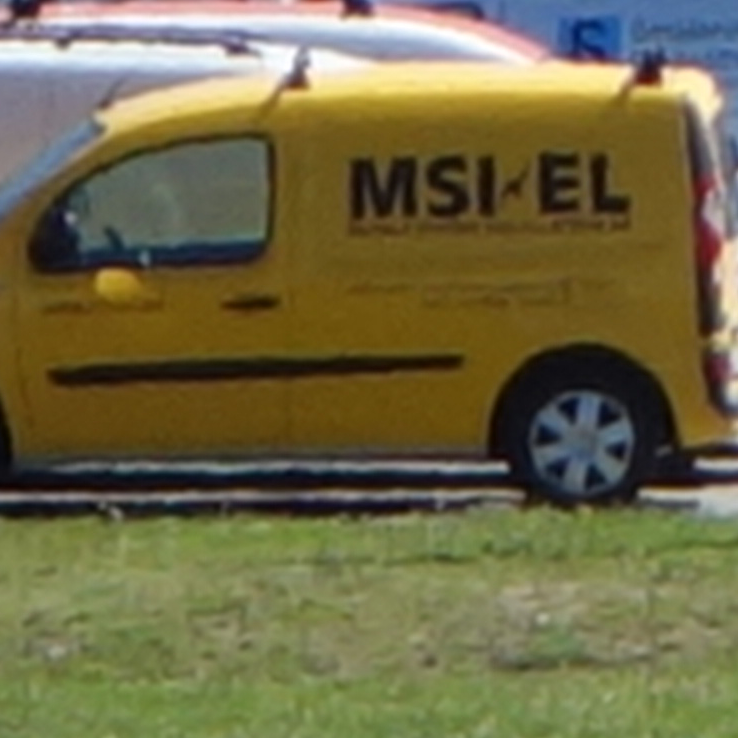
\includegraphics[width = 1\linewidth]{gfx/car/car_org.png}
	\label{fig:car_org}
\end{minipage}
\begin{minipage}[t]{0.3\linewidth} % Hus
	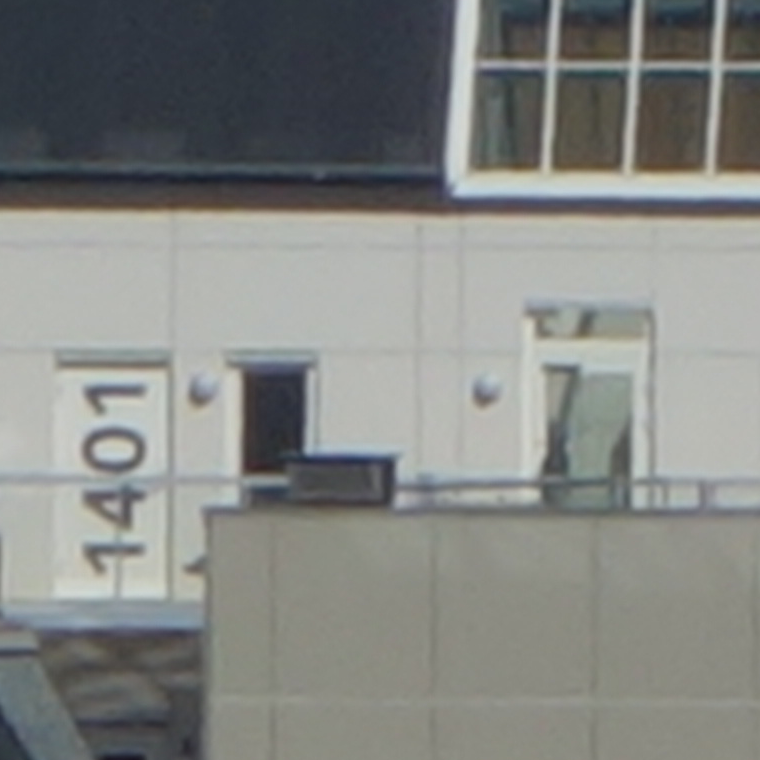
\includegraphics[width = 1\linewidth]{gfx/hus/hus_org.png}
	\label{fig:hus_org}
\end{minipage}
\begin{minipage}[t]{0.3\linewidth} %Sit
	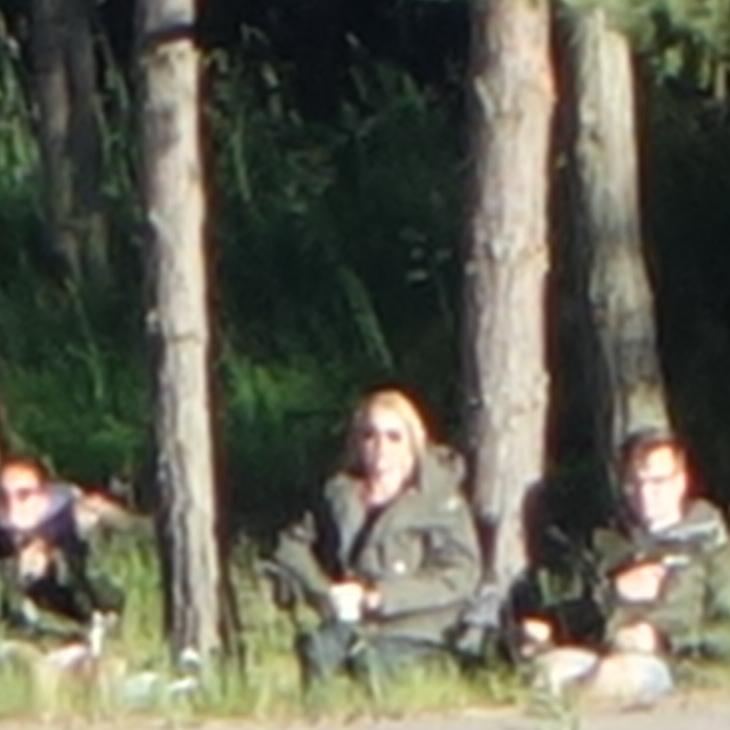
\includegraphics[width = 1\linewidth]{gfx/sit/sit_org.png}
	\label{fig:sit_org}
\end{minipage}
\end{figure}
\begin{figure}[H]
\vspace*{-1.2cm}
\begin{minipage}[t]{0.3\linewidth} %Car
	
\includegraphics[width = 1\linewidth]{gfx/car/car_m5.png}
	\label{fig:car_m5}
\end{minipage}
\begin{minipage}[t]{0.3\linewidth} % Hus
	
\includegraphics[width = 1\linewidth]{gfx/hus/hus_m5.png}
	\label{fig:hus_m5}
\end{minipage}
\begin{minipage}[t]{0.3\linewidth} %Sit
	
\includegraphics[width = 1\linewidth]{gfx/sit/sit_m10.png}
	\label{fig:sit_m5}
\end{minipage}
\end{figure}
\begin{figure}[H]
\vspace*{-1.2cm}
\begin{minipage}[t]{0.3\linewidth} %Car
	
\includegraphics[width = 1\linewidth]{gfx/car/car_m10.png}
	%\subcaption{m15}
	\label{fig:car_m10}
\end{minipage}
\begin{minipage}[t]{0.3\linewidth} % Hus
	
\includegraphics[width = 1\linewidth]{gfx/hus/hus_m10.png}
	%\subcaption{m10}
	\label{fig:hus_m10}
\end{minipage}
\begin{minipage}[t]{0.3\linewidth} %Sit
	
\includegraphics[width = 1\linewidth]{gfx/sit/sit_m10.png}
	%\subcaption{m10}
	\label{fig:sit_m10}
\end{minipage}
\end{figure}
\begin{figure}[H]
\vspace*{-1.2cm}
\begin{minipage}[t]{0.3\linewidth} %Car
	
\includegraphics[width = 1\linewidth]{gfx/car/car_m15.png}
	\subcaption{m15}
	\label{fig:car_m15}
\end{minipage}
\begin{minipage}[t]{0.3\linewidth} % Hus
	
\includegraphics[width = 1\linewidth]{gfx/hus/hus_m15.png}
	\subcaption{m10}
	\label{fig:hus_m15}
\end{minipage}
\begin{minipage}[t]{0.3\linewidth} %Sit
	
\includegraphics[width = 1\linewidth]{gfx/sit/sit_m15.png}
	\subcaption{m10}
	\label{fig:sit_m15}
\end{minipage}
\end{figure}
\begin{figure}[H]
\vspace*{-1.2cm}
\begin{minipage}[t]{0.3\linewidth} %Car
	
\includegraphics[width = 1\linewidth]{gfx/car/car_m20.png}
	%\subcaption{m15}
	\label{fig:car_m20}
\end{minipage}
\begin{minipage}[t]{0.3\linewidth} % Hus
	
\includegraphics[width = 1\linewidth]{gfx/hus/hus_m20.png}
	%\subcaption{m10}
	\label{fig:hus_m20}
\end{minipage}
\begin{minipage}[t]{0.3\linewidth} %Sit
	
\includegraphics[width = 1\linewidth]{gfx/sit/sit_m20.png}
	%\subcaption{m10}
	\label{fig:sit_m20}
\end{minipage}
\end{figure}
\begin{figure}[H]
\begin{minipage}[t]{0.3\linewidth} %Car
	
\includegraphics[width = 1\linewidth]{gfx/car/car_m25.png}
	%\subcaption{m15}
	\label{fig:car_m25}
\end{minipage}
\begin{minipage}[t]{0.3\linewidth} % Hus
	
\includegraphics[width = 1\linewidth]{gfx/hus/hus_m25.png}
	%\subcaption{m10}
	\label{fig:hus_m25}
\end{minipage}
\begin{minipage}[t]{0.3\linewidth} %Sit
	
\includegraphics[width = 1\linewidth]{gfx/sit/sit_m25.png}
	%\subcaption{m20}
	\label{fig:sit_m25}
\end{minipage}
\end{figure}
\begin{figure}[H]
\vspace*{-1.2cm}
\begin{minipage}[t]{0.3\linewidth} %Car
	
\includegraphics[width = 1\linewidth]{gfx/car/car_m30.png}
	%\subcaption{m15}
	\label{fig:car_m30}
\end{minipage}
\begin{minipage}[t]{0.3\linewidth} % Hus
	
\includegraphics[width = 1\linewidth]{gfx/hus/hus_m30.png}
	%\subcaption{m10}
	\label{fig:hus_m30}
\end{minipage}
\begin{minipage}[t]{0.3\linewidth} %Sit
	
\includegraphics[width = 1\linewidth]{gfx/sit/sit_m30.png}
	%\subcaption{m10}
	\label{fig:sit_m30}
\end{minipage}
	\caption{Images reconstructed using $M/N = 5\% \text{ to } 30\%$ measurements from top down.} 
\end{figure}

\subsubsection{Soft chessboard}
\todo[inline]{Todo: Skapa rekonstruerade bilder från homagraphin och jämnför de rekonstruerade med referensbilden}
This evaluation is designed to confirm that the images reconstructed by the SPC follows the same characteristics as the reconstruction of the synthetic data.

\begin{figure}[H]
    \centering
    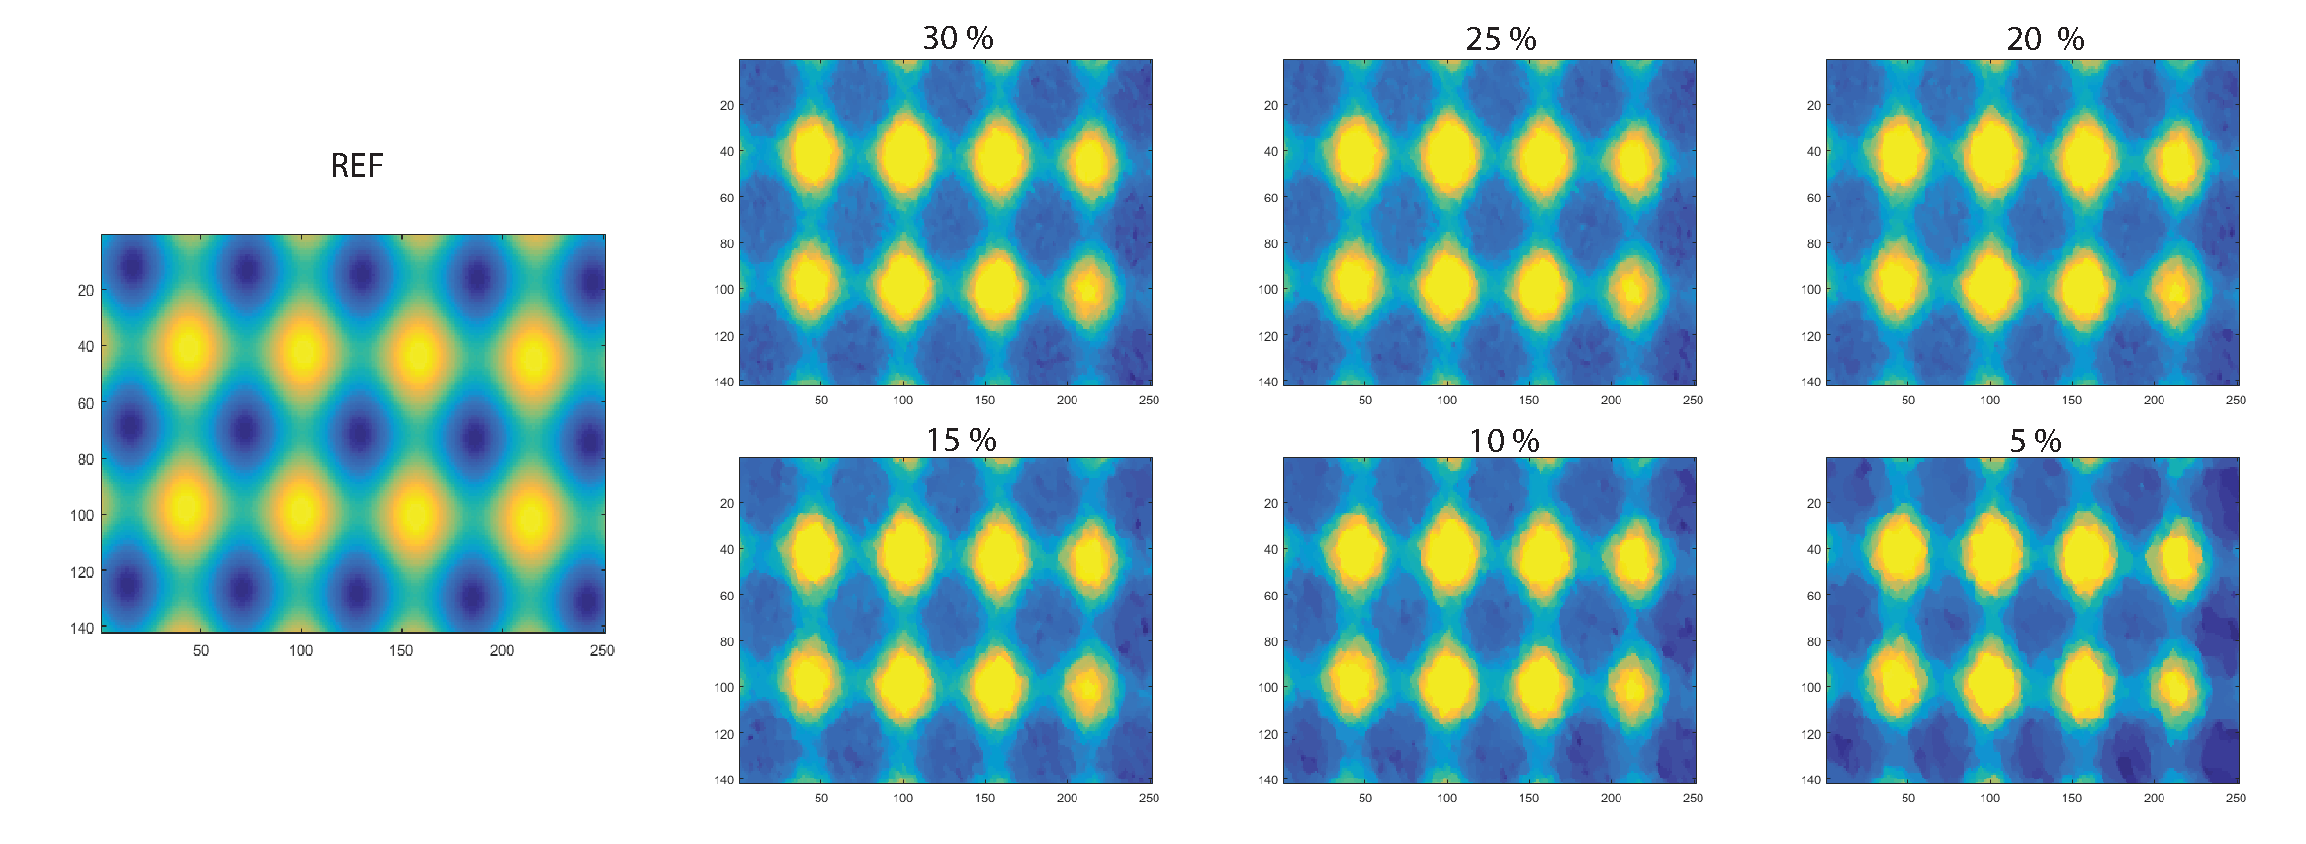
\includegraphics[width=1\linewidth]{result/homo/Hom_im.eps}
    \caption{The reconstructed images with different number of measurements and the reference image transformed to fit the SPC images using homography.}
    \label{fig:hom_over_im}
\end{figure}

\begin{figure}[H]
    \centering
\begin{minipage}[t]{0.49\textwidth}
    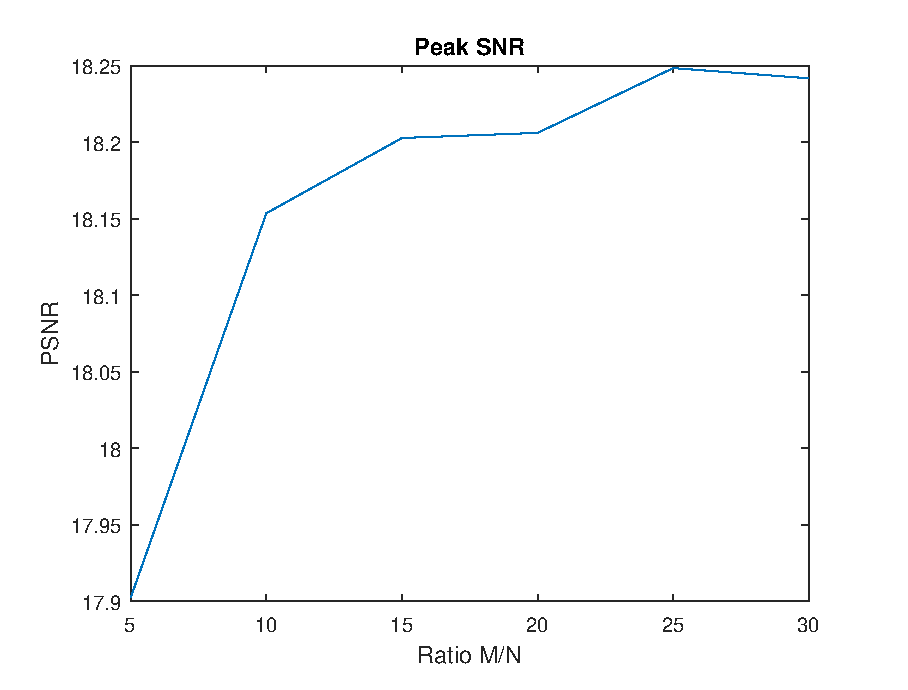
\includegraphics[width=1\textwidth]{result/homo/hom_PSNR.eps}
    \subcaption{Peak SNR for reconstructed images against reference image.}
    \label{fig:hom_psnr}
\end{minipage}
\begin{minipage}[t]{0.49\textwidth}
    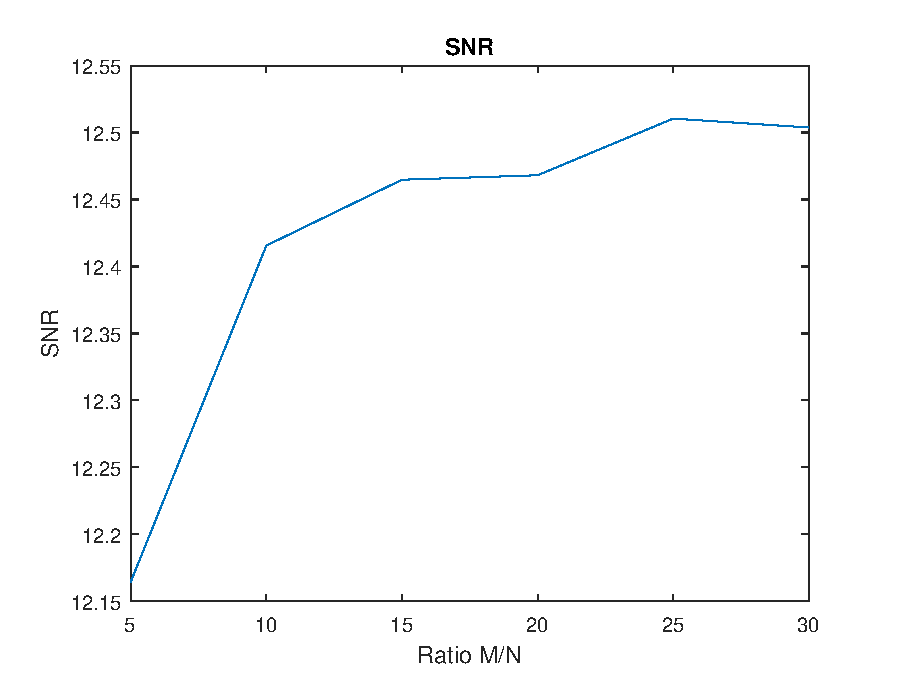
\includegraphics[width = \textwidth]{result/homo/hom_SNR.eps}
    \subcaption{SNR for reconstructed images against reference image.}
    \label{fig:hom_snr}
\end{minipage}
\begin{minipage}[t]{0.49\textwidth}
    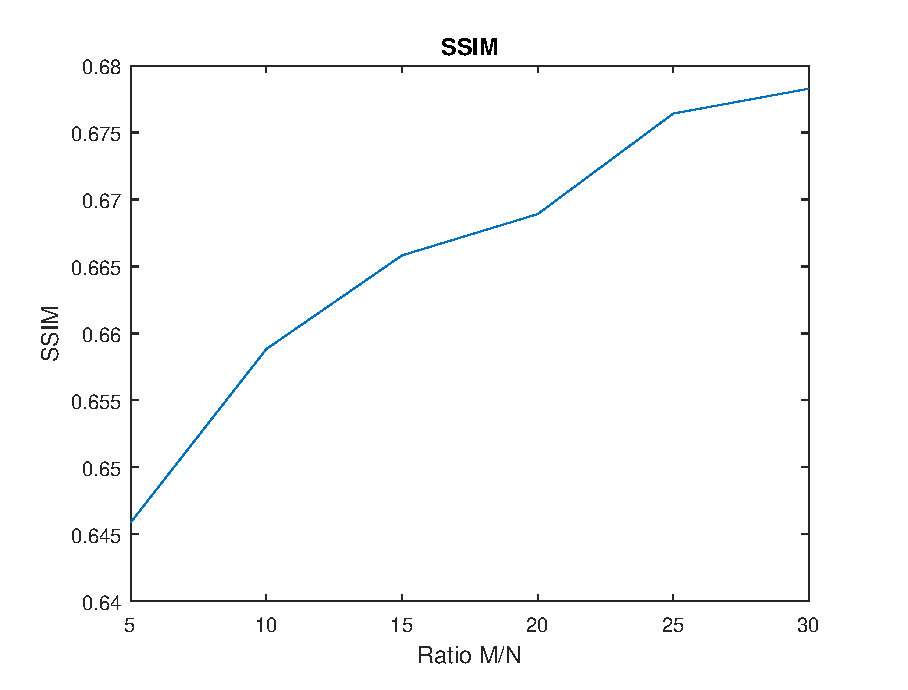
\includegraphics[width=1\textwidth]{result/homo/hom_SSIM.eps}
    \subcaption{SSIM score for reconstructed images against reference image.}
    \label{fig:hom_ssim}
\end{minipage}
    \caption{Signal quality of SPC images compared to reference image}
    \label{fig:hom_score}
\end{figure}


\subsubsection{No reference quality assessment}
Using the no reference quality assessment measurement BRISQUE to evaluate the SPC images. Each image is evaluated at reconstruction rate $5\%$ to $30\%$.

\begin{figure}[H]
    \centering
    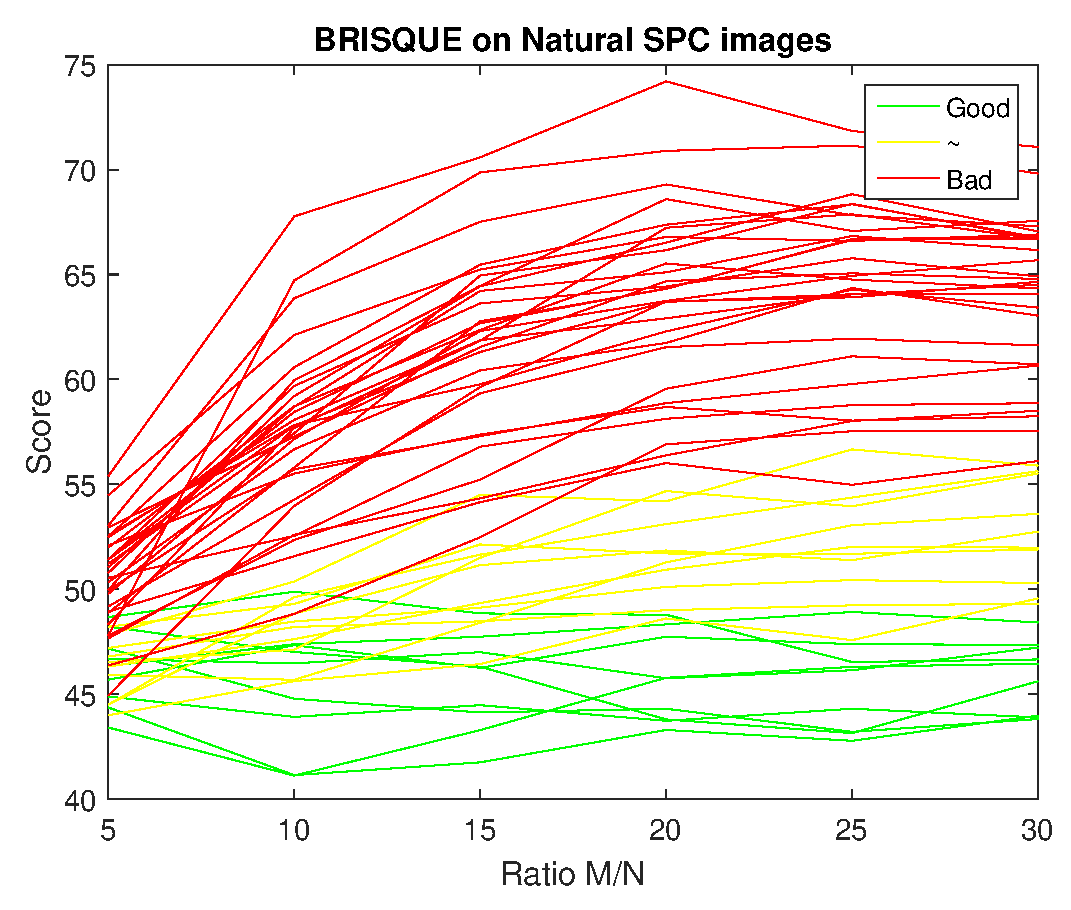
\includegraphics[width = 0.7\linewidth]{result/SPC_NRQA/plot.eps}
    \caption{BRISQUE result.}
    \label{fig:brisque_plot}
\end{figure}

\begin{figure}[H]
    \centering
    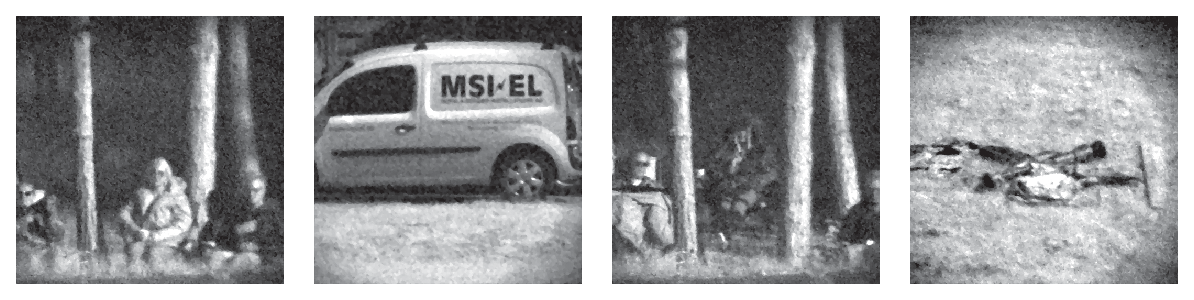
\includegraphics[width = 1\linewidth]{result/SPC_NRQA/good.eps}
    \caption{Example of 'good' images corresponding to the green lines in figure~\ref{fig:brisque_plot}.}
    \label{fig:good_plot}
\end{figure}

\begin{figure}[H]
    \centering
    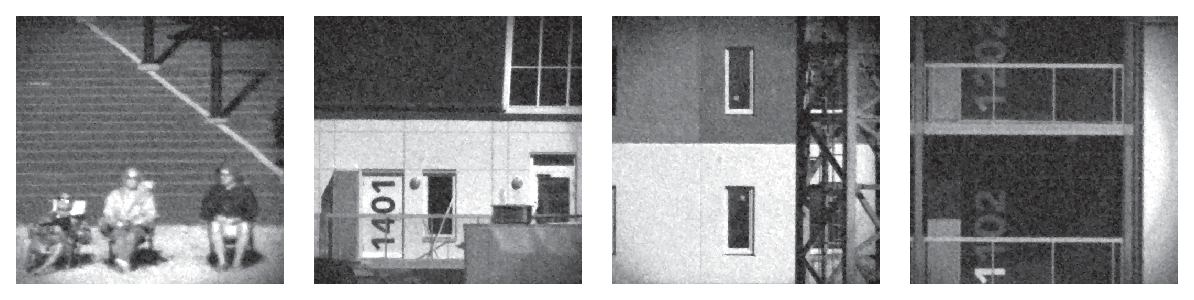
\includegraphics[width = 1\linewidth]{result/SPC_NRQA/half.eps}
    \caption{Example of 'medium good' images corresponding to the yellow lines in figure~\ref{fig:brisque_plot}.}
    \label{fig:half_plot}
\end{figure}

\begin{figure}[H]
    \centering
    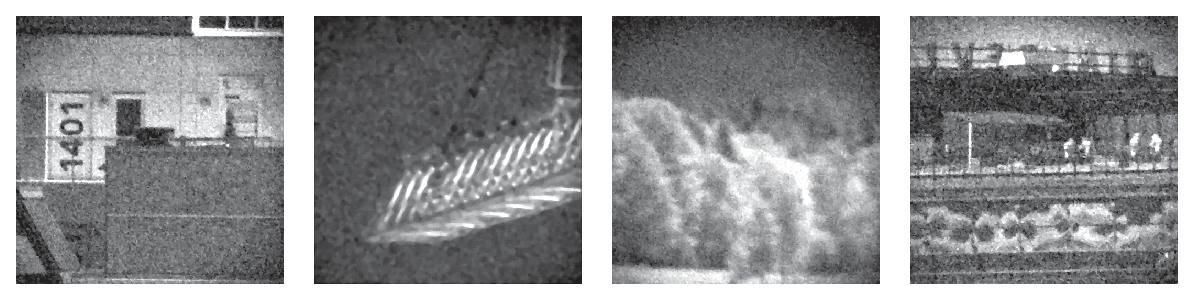
\includegraphics[width = 1\linewidth]{result/SPC_NRQA/bad.eps}
    \caption{Example of 'bad' images corresponding to the red lines in figure~\ref{fig:brisque_plot}.}
    \label{fig:bad_plot}
\end{figure}

\begin{itemize}
    \item Good images are:
    \item Medium good images are:
    \item Bad images are:
\end{itemize}


\subsubsection{Modulation Transfer Function}
The MTF is used to comparing the sharpness of cameras and lenses.  

%for two reasons: (1) Image contrast is half its low frequency or peak values,hence detail is still quite visible. The eye is relatively insensitive to detail at spatial frequencies where MTF is low: 10 or less. (2) The response of most cameras falls off rapidly in the vicinity of MTF50 and MTF50P. MTF50P is a better metric for strongly sharpened cameras that have “halos” near edges and corresponding peaks in their MTF response.

The MTF from the SPC is compared to a state of the art SWIR camera. Two scenes was captured by the SPC and a conventional SWIR camera containing printed sheath of paper with simple tilted shapes on them, see figure~\ref{fig:mtf_target}. 



\begin{figure}[H]
    \centering
    
\includegraphics[width=0.9\linewidth]{result/mtf/Target.eps}
    \caption{Printed targets with markings where the MTF measurements was performed}
    \label{fig:mtf_target}
\end{figure}

In the resulting images MTF measurements was performed on the specified edges to gather a mean and standard deviation for each camera. For the SPC, images reconstructed from 5\% to 30\% was tested in order to see if the number of measurements effected the MTF result. In figure~\ref{fig:mtf_target_im} the images from the SWIR camera and SPC are presented.

\begin{figure}[H]
    \centering
    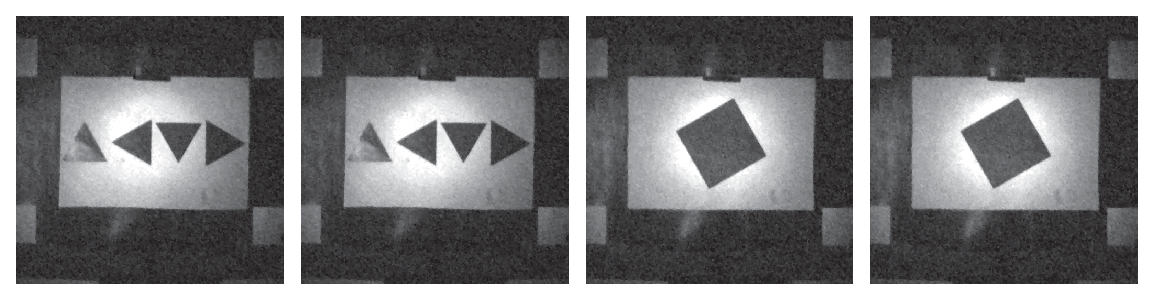
\includegraphics[width=1\linewidth]{result/mtf/Target_im.eps}
    \caption{SPC and state of the art SWIR camera output images. (OBS! Bilder från Raptorn ska läggas till)}
    \label{fig:mtf_target_im}
\end{figure}


\subsection{MTF}


\begin{figure}[H]
    \centering
    \begin{minipage}{0.49\textwidth}
    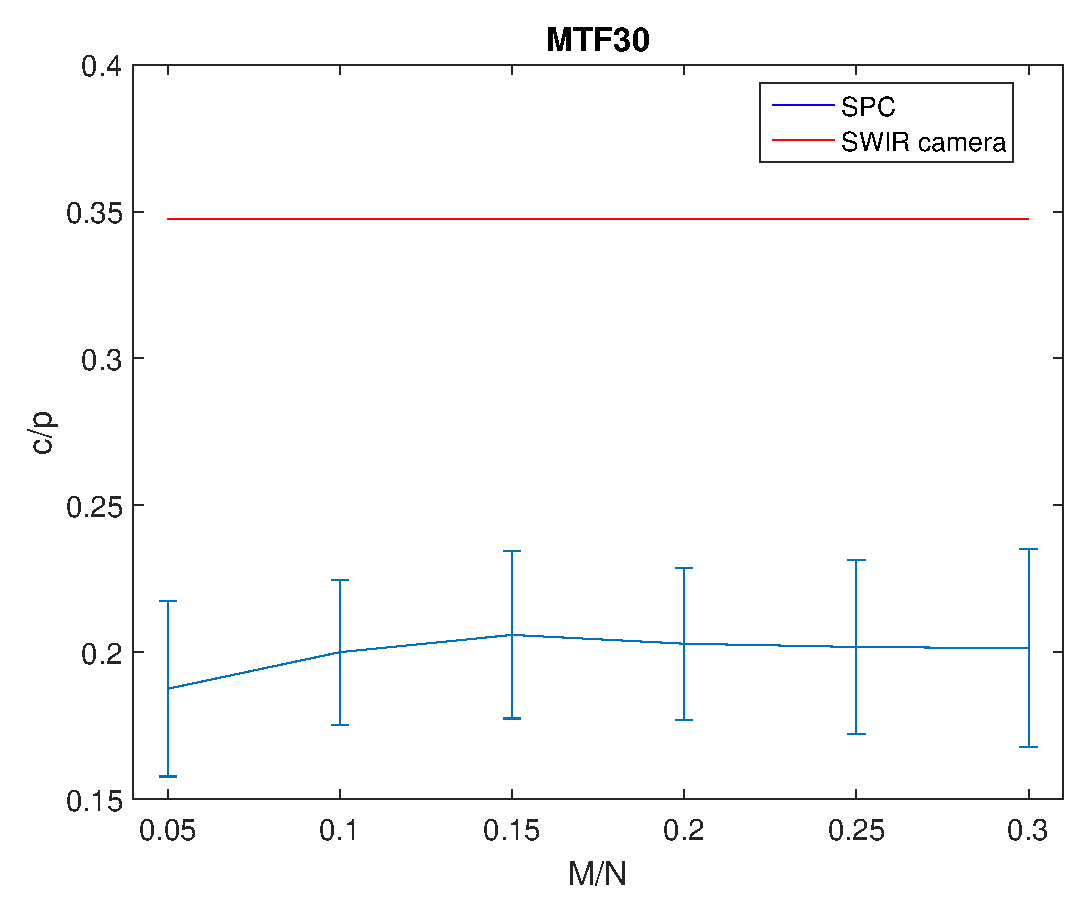
\includegraphics[width=1\textwidth]{result/mtf/mtf30.eps}
    \subcaption{MTF30 result.}
    \label{fig:mtf30}
\end{minipage}
\begin{minipage}{0.49\textwidth}
    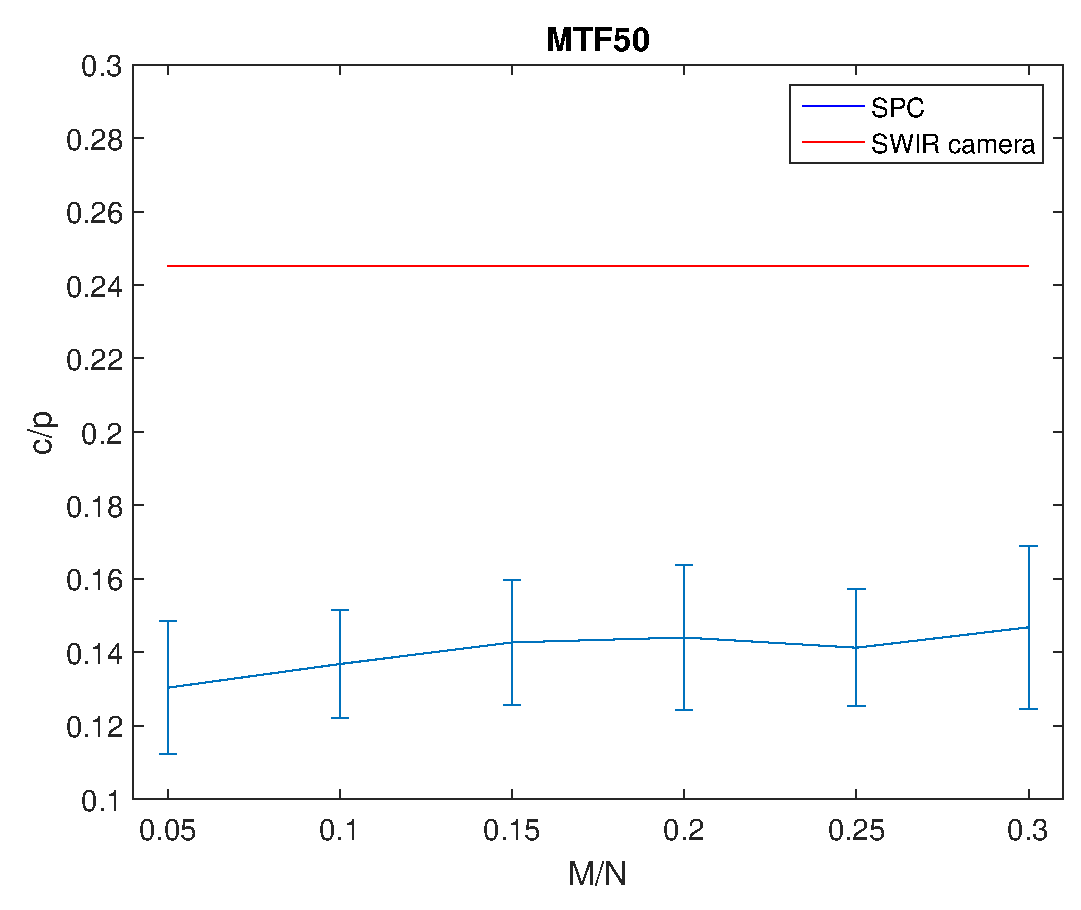
\includegraphics[width = \textwidth]{result/mtf/mtf50.eps}
    \subcaption{MTF50 result.}
    \label{fig:i2}
\end{minipage}
    \caption{MTF results. (OBS! inte rätt figurer)}
    \label{fig:mtf50}
\end{figure}

\subsection{Edge response}
The edge response is measured in the distance (pixels) required for the edge to rise from $10\%$ to $90\%$. In figure~\ref{fig:rise} the result from the experiment in presented. 

\begin{figure}[H]
    \centering
    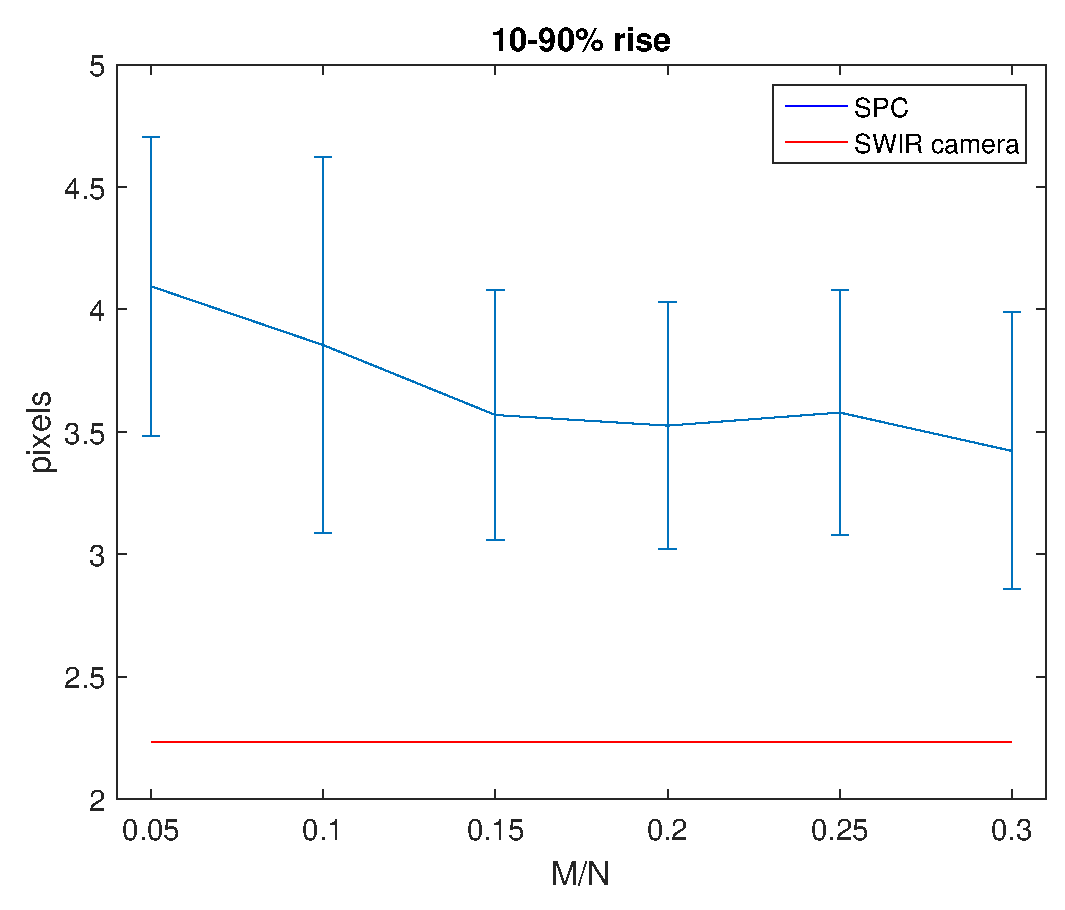
\includegraphics[width=0.5\linewidth]{result/mtf/10-90_rise.eps}
    \caption{10-90\% rise in pixels. (OBS! inte rätt figur)}
    \label{fig:rise}
\end{figure}

